\documentclass[table,aspectratio=169]{beamer}
%% Choose aspect ratio:
% [aspectratio=43]  % 4:3 (default)
% [aspectratio=169] % 16:9, wide

\usetheme[minimal, nofont, noheadline]{tugraz2018}
%\usetheme[iaik,]{tugraz2018}
%% Choose main theme variant:
% [standard]        % standard (default)
% [iaik]       % with institute's graphical acronym on the left
% [minimal]         % with reduced visuals

%% Choose your font style:
%                   % Helvetica (default for Corporate Design)
% [webfont]         % Source Sans Pro (as used on tugraz.at)
% [nofont]          % no font loaded - Computer Modern Sans

%% Choose your department's color instead of TU Graz red (optional):
% [arch]            % 
% [bau]             %
% [etit]            %
% [mbww]            %
% [tcvp]            %
% [mpug]            %
% [infbio]          %


\usepackage[utf8]{inputenc}
\usepackage[english]{babel}
%% Choose your language:
% [ngerman]   % German
% [english]   % English


%% Add your own packages, macros, etc.
\usepackage{xcolor,colortbl}
\usepackage{booktabs,nicematrix}
\usepackage{rotating}
\usepackage[style=alphabetic,backend=biber]{biblatex} % Bibliography
\addbibresource{\jobname.bib}                         % Bibliography
\usepackage{fontawesome}
\usepackage{filecontents}
\usepackage{setspace}
\usepackage{subcaption}
\usepackage{multirow}
\usepackage{bm}
\usepackage{pgfplots}
\usepackage[linesnumbered,ruled,vlined]{algorithm2e}

\tikzset{
  invisible/.style={opacity=0},
  visible on/.style={alt={#1{}{invisible}}},
  alt/.code args={<#1>#2#3}{%
    \alt<#1>{\pgfkeysalso{#2}}{\pgfkeysalso{#3}} % \pgfkeysalso doesn't change the path
  },
}

\usetikzlibrary{calc,patterns,arrows.meta, shapes.geometric}
\usetikzlibrary{positioning}
\usetikzlibrary{cipher}
\setbeamersize
{
	text margin left=0.4cm,
	text margin right=0.4cm
}

%% Enter presentation metadata
\title{Practical Multiple Persistent Fault Analysis}
\author{Hadi Soleimany \and Nasour Bagheri \and \underline{\textbf{Hosein Hadipour}} \and Prasanna Ravi \and Shivam Bhasin \and Sara Mansouri}
\date{CHES 2022 - Leuven, Belgium}
%\institute{IAIK}
\instituteurl{hsn.hadipour@gmail.com}

%% Logos
%\institutelogo{beamerthemetugraz/institute/IAIK}  % graphical acronym for [] theme (left margin)
% \additionallogo{figures/logo}  % additional institute/department logo (footline; optional)
% \logobar{Supported by: ...}  % sponsors (titlepage; optional)

%% Macros
\definecolor{gold}{HTML}{F0AB00}
\definecolor{bound}{HTML}{78b473}
\definecolor{best}{HTML}{e59352}
\definecolor{lin}{HTML}{285f82}
\definecolor{sub}{HTML}{78b473}
\definecolor{lightred}{rgb}{0.9, 0.2, 0.2}
\definecolor{lightblue}{rgb}{0, 0.5, 0.9}

\newcommand{\sparen}{\vspace*{-.3cm}}
\newcommand{\cipher}[1]{\textsc{#1}}

\begin{document}

\begin{frame}[plain]
  \maketitle
\end{frame}


\section*{}
\begin{frame}{Outline}
  \tableofcontents
\end{frame}

\section{Introduction and the Research Gap}
\sectionheader[\huge\color{tug}\faBook]{Introduction and the Research Gap}

\begin{frame}{Fault Attacks}
\begin{itemize}
\item[\faWarning] \textbf{Fault attack}: An active side-channel attack \cite{eurocrypt_BonehDL97}:
\begin{itemize}
	\item[\faMagic]<1-> \textbf{Fault injection}: Disturb the operation of a cryptographic device	
	\item[\faLaptop]<2-> \textbf{Fault analysis}: Analyze the erroneous outputs to retrieve the secret key
\end{itemize}
\end{itemize}
\begin{figure}
\centering
\only<1>{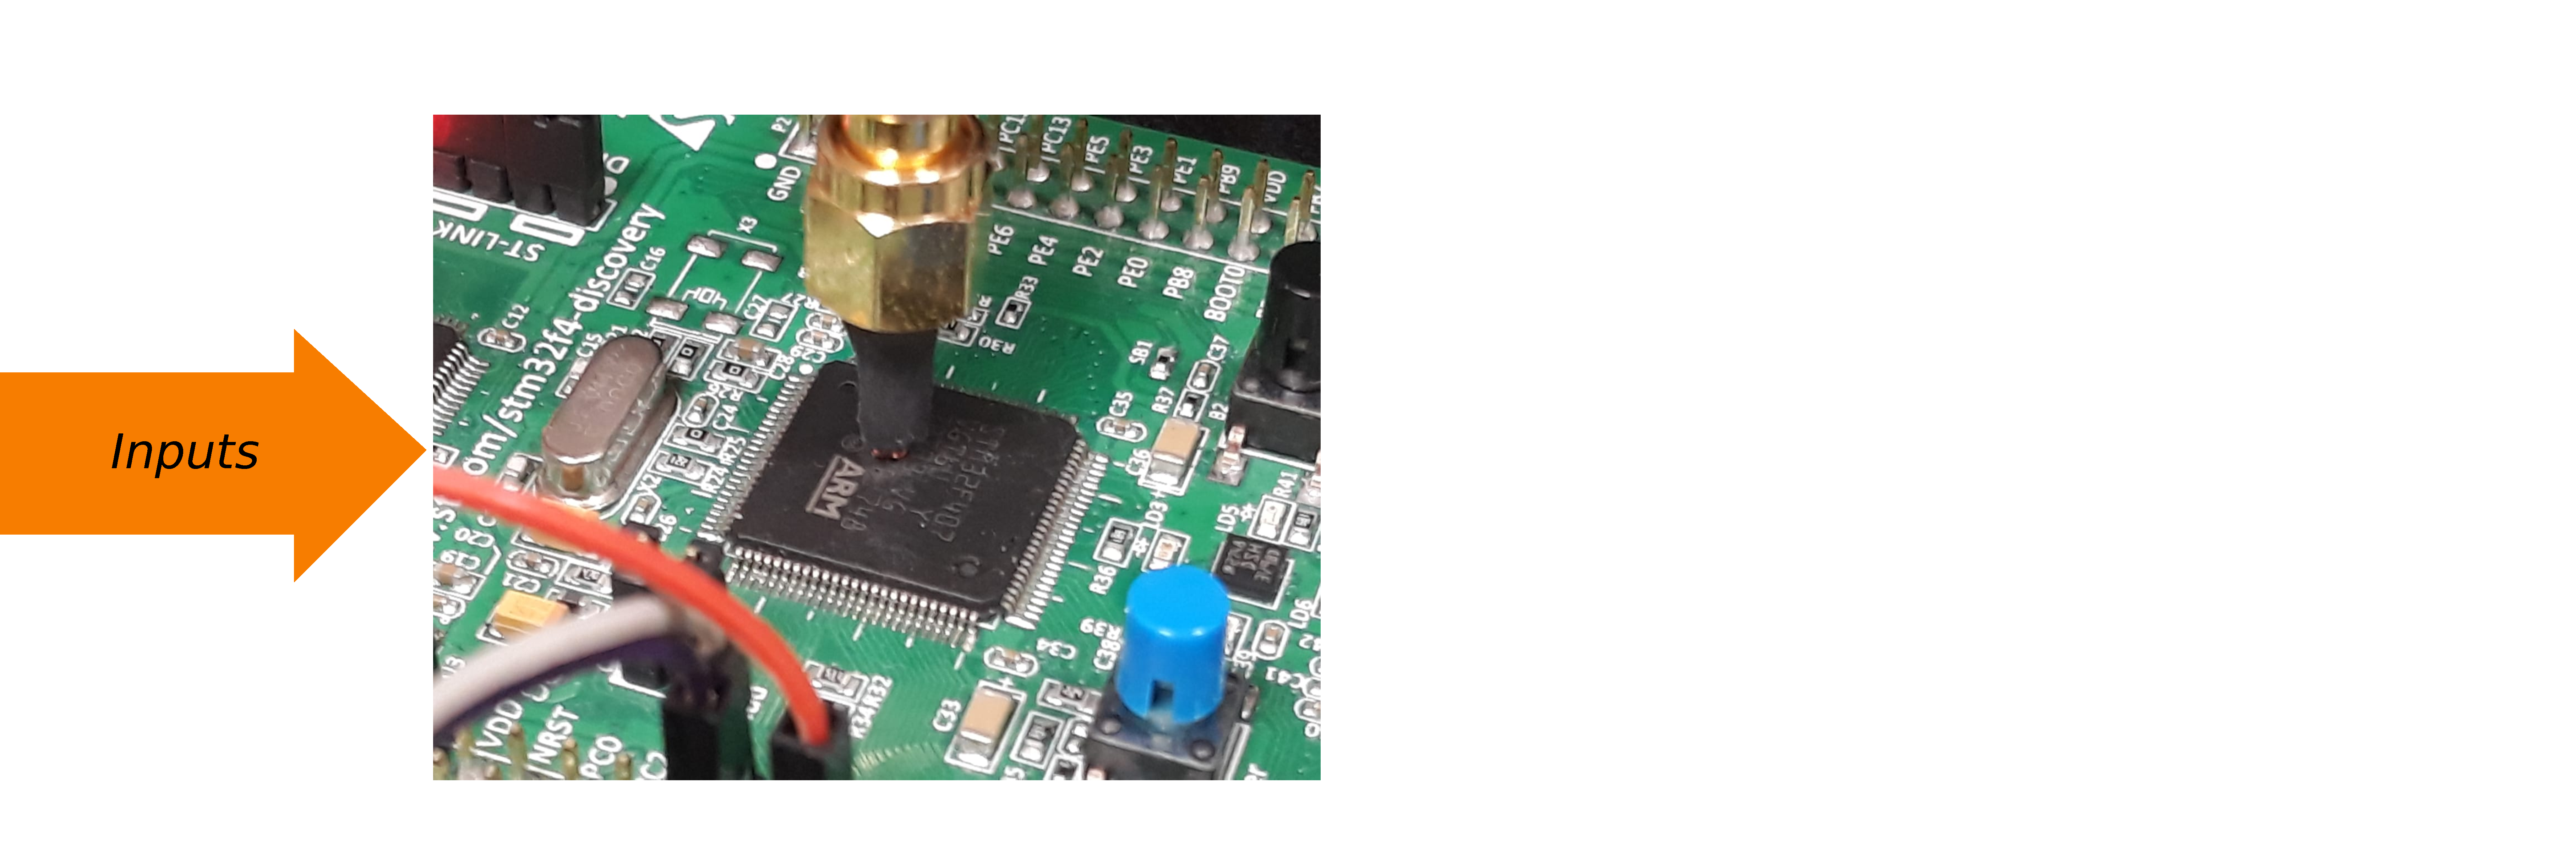
\includegraphics[width=0.7\textwidth]{./figures/fa1.pdf}}
\only<2>{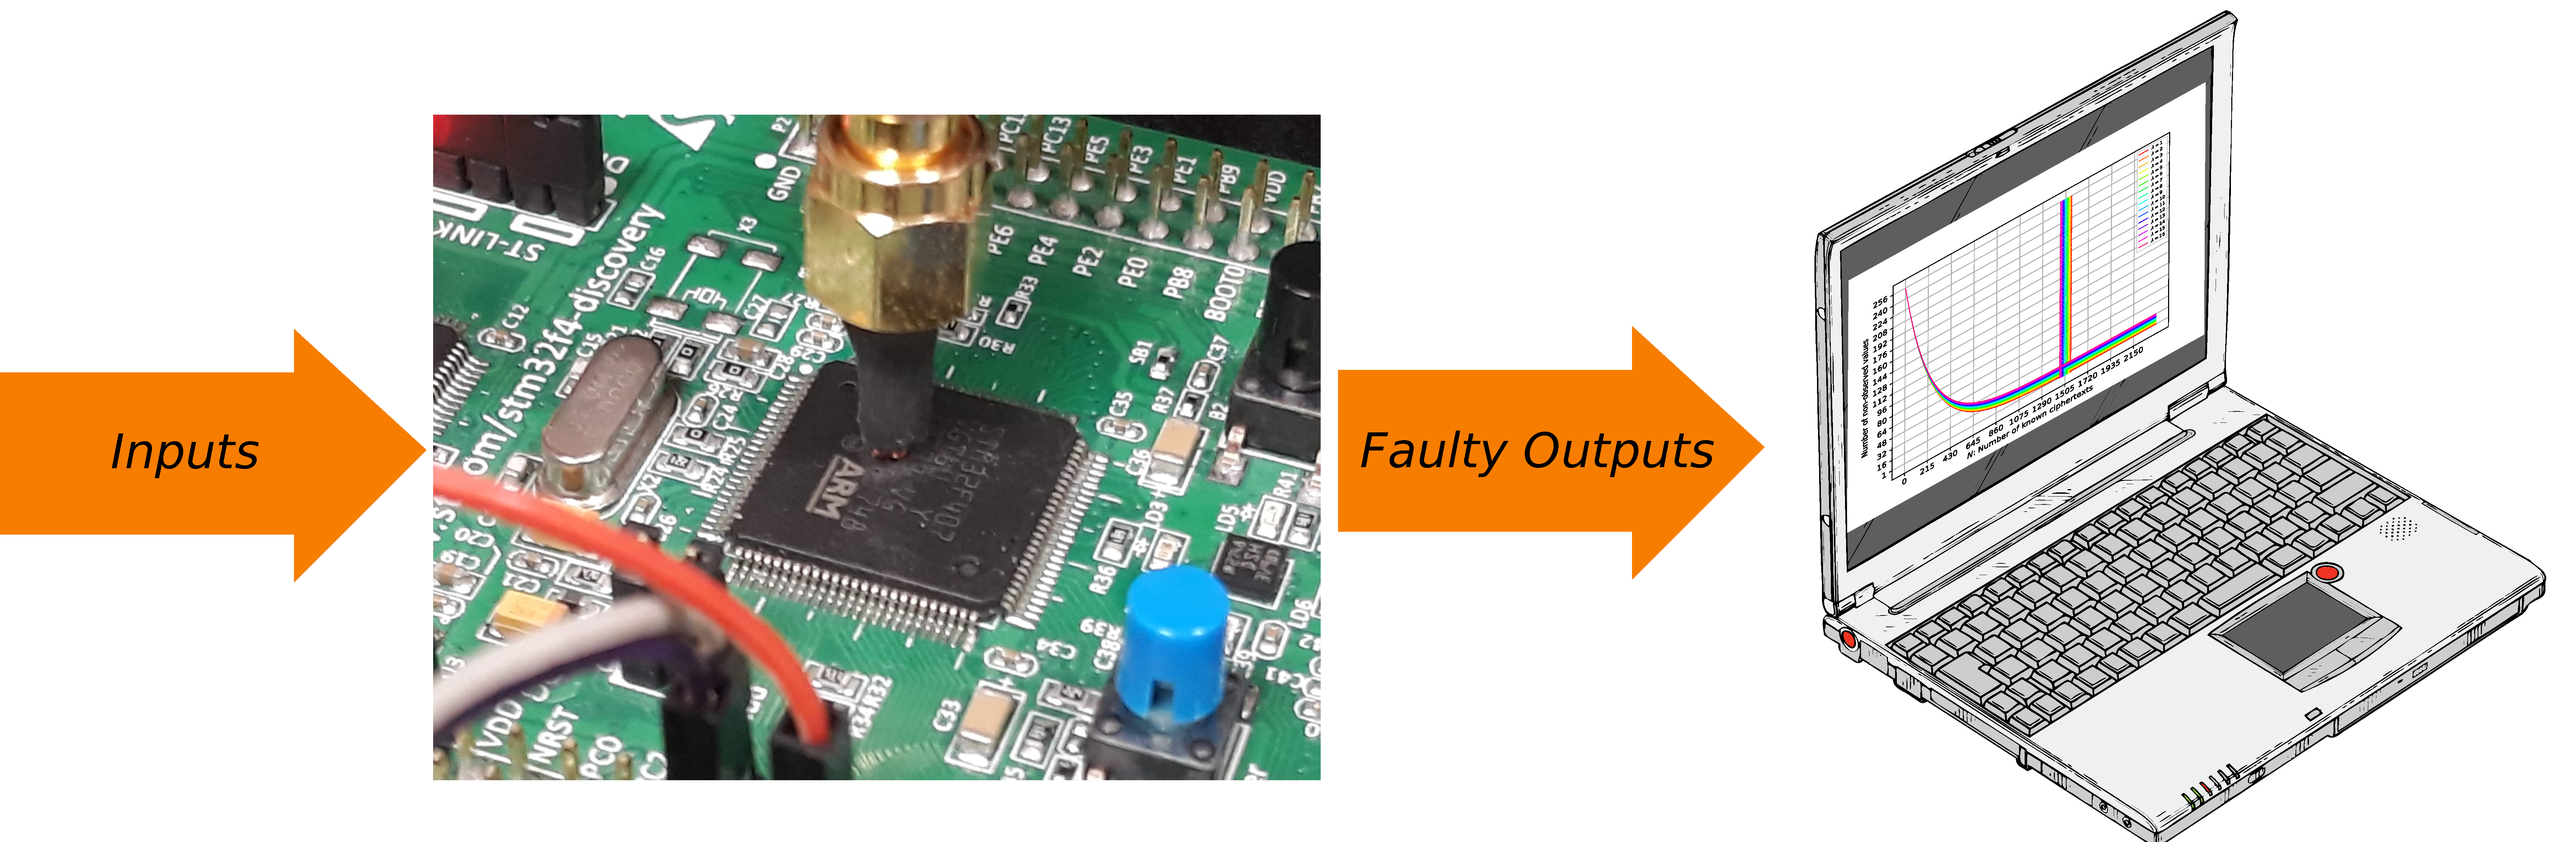
\includegraphics[width=0.7\textwidth]{./figures/fa2.pdf}}
\end{figure}
\end{frame}

\begin{frame}{Persisent Fault Attack (PFA)}
PFA fault model\cite{tches_0010L0BHDQR18}:
\begin{itemize}
\item<1-> We can inject the faults before the encryption
\item<2-> The injected faults typically alter the stored algorithm constants
\item<3-> The injected faults are persistent until the reset of the device
\item<4-> We can collect multiple faulty ciphertexts
\end{itemize}
\onslide<2->{
\begin{center}
  \setlength\extrarowheight{0.2ex}
  \scalebox{0.8}{
    \begin{tabular}{|c|c|c|c|c|c|c|c|c|c|c|c|c|c|c|c|c|}
      \hline
      $x$   & $\mathtt 0$ & $\mathtt 1$ & $\mathtt 2$ & $\mathtt 3$ & $ \mathtt 4$ & $\mathtt 5$ & $\mathtt 6$ & $\mathtt 7$ & $ \mathtt 8$ & $\mathtt 9$ & $\mathtt a$ & $\mathtt b$ & $\mathtt c$ & $\mathtt d$ & $\mathtt e$ & $\mathtt f$ \\
      \hline
      $\mathcal S(x)$ & $\mathtt 6$ & $\mathtt 4$ & $\mathtt  c$ & $\mathtt 5$ & $\mathtt 0$ & $\mathtt 7$ & $\mathtt 2$ & \cellcolor{tugred} $\mathtt e$ & $\mathtt 1$ & $\mathtt f$ & $\mathtt 3$ & $\mathtt d$ & $\mathtt 8$ & $\mathtt a$ & $\mathtt 9$ & $\mathtt b$\\
      \hline
      \hline
      $\mathcal S'(x)$ & $\mathtt 6$ & $\mathtt 4$ & $\mathtt  c$ & $\mathtt 5$ & $\mathtt 0$ & $\mathtt 7$ & $\mathtt 2$ & \cellcolor{tugred} $\mathtt 4$ & $\mathtt 1$ & $\mathtt f$ & $\mathtt 3$ & $\mathtt d$ & $\mathtt 8$ & $\mathtt a$ & $\mathtt 9$ & $\mathtt b$\\
      \hline
    \end{tabular}
  }
\end{center}
}
\end{frame}

\begin{frame}{Core Idea of PFA}
\vspace{-0.2cm}
\begin{columns}[onlytextwidth]
\column[c]{0.7\textwidth}
\begin{center}
\scalebox{0.8}{
  \begin{tabular}{|c|c|c|c|c|c|c|c|c|c|c|c|c|c|c|c|c|}
    \hline
    $x$   & $\mathtt 0$ & $\mathtt 1$ & $\mathtt 2$ & $\mathtt 3$ & $ \mathtt 4$ & $\mathtt 5$ & $\mathtt 6$ & $\mathtt 7$ & $ \mathtt 8$ & $\mathtt 9$ & $\mathtt a$ & $\mathtt b$ & $\mathtt c$ & $\mathtt d$ & $\mathtt e$ & $\mathtt f$ \\
    \hline
    $\mathcal S(x)$ & $\mathtt 6$ & $\mathtt 4$ & $\mathtt  c$ & $\mathtt 5$ & $\mathtt 0$ & $\mathtt 7$ & $\mathtt 2$ & \cellcolor{tugyellow}{$\mathtt e$} & $\mathtt 1$ & $\mathtt f$ & $\mathtt 3$ & $\mathtt d$ & $\mathtt 8$ & $\mathtt a$ & $\mathtt 9$ & $\mathtt b$\\
    \hline
  \end{tabular}
}
\[c = S(x) + \textcolor{tugred}{k}\]
\end{center}

\onslide<2->{
\begin{center}
\scalebox{0.8}{
  \begin{tabular}{|c|c|c|c|c|c|c|c|c|c|c|c|c|c|c|c|c|}
    \hline
    $x$   & $\mathtt 0$ & $\mathtt 1$ & $\mathtt 2$ & $\mathtt 3$ & $\mathtt 4$ & $\mathtt 5$ & $\mathtt 6$ & $\mathtt 7$ & $\mathtt 8$ & $\mathtt 9$ & $\mathtt a$ & $\mathtt b$ & $\mathtt c $&$ \mathtt d$ &$ \mathtt e$ &$ \mathtt f$ \\
    \hline
    $\mathcal S'(x)$ & $\mathtt 6$ & $\mathtt 4$ & $\mathtt  c$ & $\mathtt 5$ & $\mathtt 0$ & $\mathtt 7$ & $\mathtt 2$ & \cellcolor{tugyellow}{$\mathtt 4$} & $\mathtt 1$ & $\mathtt f$ &$\mathtt  3$ &$\mathtt d $&$\mathtt 8$ & $\mathtt a$ & $\mathtt 9$ & $\mathtt b$\\
    \hline
  \end{tabular}
}
\[c = S'(x) \oplus \textcolor{tugred}{k}\]
\end{center}
}
\vspace{-0.2cm}
\begin{itemize}
  \item<3> \textcolor{tugblue}{Filter wrong keys}: $S'(x) \neq \texttt{0xe} \Rightarrow \textcolor{tugred}{k} \neq \texttt{0xe} \oplus c$
  \vspace{-0.2cm}
  \item<4> \textcolor{tugblue}{Filter wrong keys}: $S'(X[i]) \neq \texttt{0xe} \Rightarrow \textcolor{tugred}{K[i]} \neq \texttt{0xe} \oplus C[i]$
\end{itemize}

\column[c]{0.3\textwidth}
\begin{center}
\only<1-3>{
\begin{tikzpicture}[very thick, >=latex, xscale=1, yscale=1]
  \pgfmathsetmacro{\esep}{0.7}
  \node (x) at (0,0) {$x$};
  \node[box, below=\esep of x] (sbox) {\only<1>{$S$}\only<2->{$S'$}};
  \node[xor, below=\esep of sbox] (xor) {};
  \node[left=\esep of xor] (k) {\textcolor{tugred}{$k$}};
  \node[below=\esep of xor] (c) {$c$};
  \draw[->] (x) -- (sbox);
  \draw[->] (sbox) --node[anchor=west] {$y\visible<2->{\neq \texttt{0xe}}$} (xor);
  \draw[->] (xor) -- (c);
  \draw[->] (k) -- (xor);
\end{tikzpicture}
}
\only<4>{
\begin{tikzpicture}[>=latex]
\draw[every node/.style={state}]
(0, 0) node (S0) {\State{\FillState[tugblue]}}
++(0, -2) node (S1) {\State{\FillState[tugblue]}}
++(0, -2.5) node (S2) {\State{\FillState[tugblue]}};
\node[xor, below=0.5cm of S1] (xor) {};
\node[left=0.5cm of xor, style={state}] (k) {\State{\FillState[tugred]}};
\draw[->] (S0) --node[anchor=west] {\texttt{SB}} (S1);
\draw[->] (S1) -- (xor);
\draw[->] (k) -- (xor);
\draw[->] (xor) -- (S2);
\draw (S0.east) node[right] {$X$};
\draw (S1.east) node[right] {$Y$};
\draw (S2.east) node[right] {$C$};
\draw (k.north) node[above] {$K$};
\end{tikzpicture}
}
\end{center}
\end{columns}
% \begin{itemize}
% 	\item PFA is a ciphertext-only Attack
% 	\item The fault injection does not require precise time synchronization with the encryption
% 	\item PFA can bypass some redundancy-based countermeasures
% \end{itemize
\end{frame}

\begin{frame}{Limits if the Original PFA}
The original PFA requires about 2000 faulty ciphertexts per key \cite{tches_0010L0BHDQR18}
\begin{columns}[onlytextwidth]
\column[c]{0.6\textwidth}
\begin{figure}
\centering
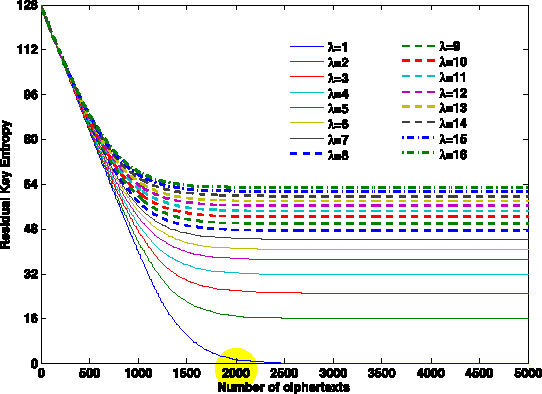
\includegraphics[width=0.8\textwidth]{./figures/pfa_residual_keys.pdf}
\end{figure}
\column[c]{0.4\textwidth}
\begin{tikzpicture}[very thick, >=latex, xscale=0.6, yscale=0.6]
\pgfmathsetmacro{\esep}{0.7}
\node (x) at (0,0) {$x$};
\node[box, below=\esep of x] (sbox) {$S'$};
\node[xor, below=\esep of sbox] (xor) {};
\node[left=\esep of xor] (k) {\textcolor{tugred}{$k$}};
\node[below=\esep of xor] (c) {$c$};
\draw[->] (x) -- (sbox);
\draw[->] (sbox) --node[anchor=west] {$\neq v$} (xor);
\draw[->] (xor) -- (c);
\draw[->] (k) -- (xor);
\draw[visible on=<1>] (c.south) node[below] {$S'(x) \neq v \Rightarrow \textcolor{tug}{k} \neq c \oplus v$};
\draw[visible on=<2>] (c.south) node[below] {$\lambda = 12 \Rightarrow \textcolor{tugred}{|\text{Keys}| = 12^{16} \approx 2^{57.36}}$};
\end{tikzpicture}
\end{columns}
\end{frame}

\begin{frame}{Limits of PFA and Its Enhanced Versions}
\begin{itemize}
\item<1-> The \textcolor{tug}{location of the injected} fault is supposed to be known
\item<2-> For multiple fault injections:
\begin{itemize}
  \item We need a known plaintext/ciphertext pair to detect the correct key
\end{itemize}
\item<3-> PFA only exploits the fault leakage in the last round
\item<4-> Enhanced PFA (EPFA) \cite{tcad_XuZYZHR21} exploits the fault leakage in multiple rounds
\item<5-> However, EPFA is not clear about exploiting multiple faults in deeper rounds
\item<6-> Morever, EPFA still relies on the assumption of knowing the \textcolor{tug}{fault location}
\end{itemize}
\end{frame}

\section{Our Framework for PFA with Multiple Faults}
\sectionheader[\huge\color{tug}\faBook]{Our Framework for PFA with Multiple Faults}

% \begin{frame}{Our Fault Model}
% \begin{itemize}
% \item<1-> The targeted implementation employs a stored lookup table for S-boxes 
% \item<2-> We inject the fault on the S-box lookup table before the encryption
% \item<3-> We have not to control the number of injected faults
% \item<4-> We remove the assumption of knowing the fault location
% \item<5-> We can collect multiple faulty ciphertexts per key
% \end{itemize}
% \end{frame}

\begin{frame}{Some Notations}
\begin{columns}[onlytextwidth]
\column[c]{0.65\textwidth}
\begin{flushleft}
\begin{itemize}
  \item<1-> $V$: Impossible values in the output of faulty S-box
  \item<2-> $D[i]$: Impossible values in the $i$th word of ciphertext
  \item<3-> $V = \textcolor{tug}{K[0]} \oplus D[0]$
  \item<3-> $D[i] = V \oplus \textcolor{tug}{K[i]}$ for all $i \in {1, \dots, 15}$
  \item<4-> $D[i] = (\textcolor{tug}{K[0]} \oplus \textcolor{tug}{K[i]}) \oplus D[0]$
  \item<4-> $\textcolor{tug}{\delta[i]} = \textcolor{tug}{K[0]} \oplus \textcolor{tug}{K[i]}$
\end{itemize}
\end{flushleft}
\column[c]{0.35\textwidth}
\begin{center}
\begin{tikzpicture}[very thick, >=latex]
  \pgfmathsetmacro{\esep}{0.7}
  \node (x) at (0,0) {$X[i]$};
  \node[box, below=\esep of x] (sbox) {$S'$};
  \node[xor, below=\esep of sbox] (xor) {};
  \node[left=\esep of xor] (k) {\textcolor{tug}{$K[i]$}};
  \node[below=\esep of xor] (c) {$\only<1-3>{\neq} D[i]$};
  \draw[->] (x) -- (sbox);
  \draw[->] (sbox) --node[anchor=west] {$\!\visible<1-4>{\neq} V$} (xor);
  \draw[->] (xor) -- (c);
  \draw[->] (k) -- (xor); 
\onslide<3->{
  \node (x) at (-2.4,0) {$X[0]$};
  \node[box, below=\esep of x] (sbox) {$S'$};
  \node[xor, below=\esep of sbox] (xor) {};
  \node[left=\esep of xor] (k) {\textcolor{tug}{$K[0]$}};
  \node[below=\esep of xor] (c) {$\only<1-3>{\neq} D[0]$};
  \draw[->] (x) -- (sbox);
  \draw[->] (sbox) --node[anchor=west] {$\!\visible<1-4>{\neq} V$} (xor);
  \draw[->] (xor) -- (c);
  \draw[->] (k) -- (xor);
  \draw[dashed, <->, visible on=<4->] (c) --node[below] {\textcolor{tug}{$\delta[i]$}} ++(2, 0);
}
\end{tikzpicture}
\end{center}
\end{columns}
\end{frame}

\begin{frame}{Number of Required Ciphertexts}
\vspace{-0.4cm}
\begin{columns}[onlytextwidth]
\column[c]{0.5\textwidth}
\centering
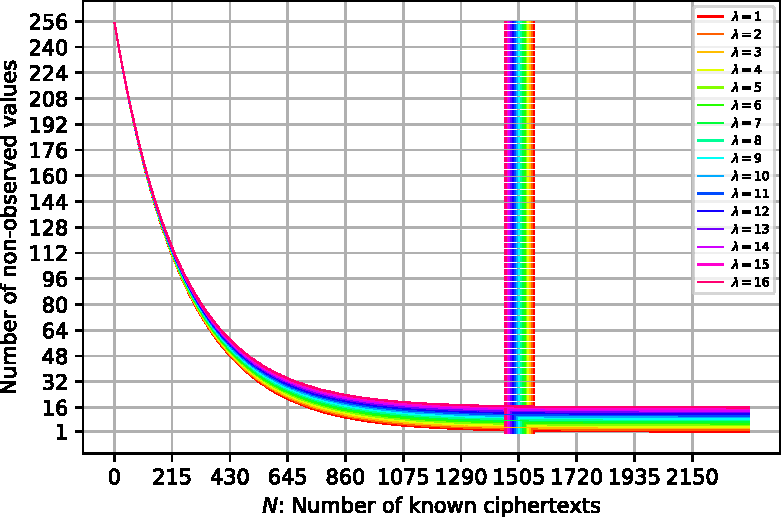
\includegraphics[width=0.77\textwidth]{./figures/overview_diagram_of_non_observed_values.pdf}
\column[c]{0.5\textwidth}
\centering
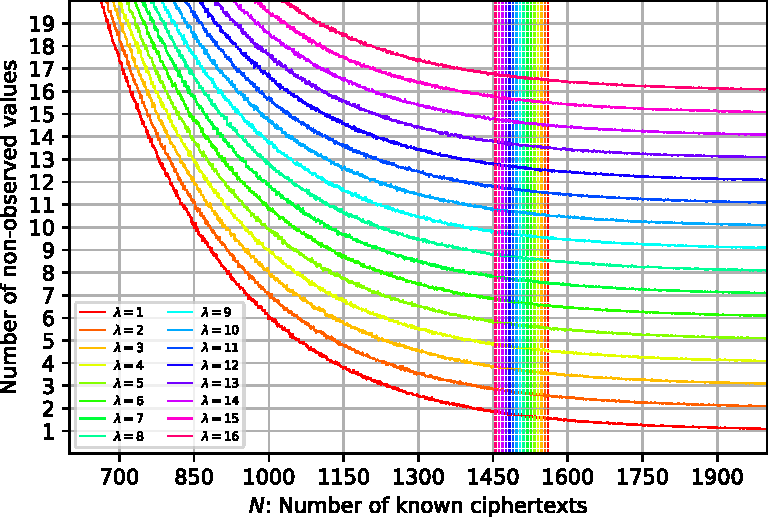
\includegraphics[width=0.77\textwidth]{./figures/close_up_diagram_of_non_observed_values.pdf}
\end{columns}
\begin{block}{Lemma}
\footnotesize
Assume that the number of injected faults is $\lambda$. 
Given $N$ faulty ciphertexts, the number of non-observed values in each word of ciphertext is
$\lambda' = \left(2^{c} - \lambda\right) e^{-\left(\frac{1}{2^{c} - \lambda}\right)\cdot N} + \lambda$, where $c$ is the cell size (8 for AES).
\end{block}
\end{frame}

\begin{frame}{\textbf{Core Idea} to Reduce the Number of Key Candidates}
\begin{center}
\begin{tikzpicture}[very thick, >=latex]
\pgfmathsetmacro{\esep}{0.7}
\foreach \i in {0,...,6}{  
  \pgfmathtruncatemacro{\sn}{(\i + 1)};
  \visible<\sn>{
  \draw[style={state}] (-2, -1) node (S0) {\State{\FillCell[tugred]{s0}, \FillCell[tugblue]{s\sn}}};
  \node (x0) at (0, 0) {$X[0]$};
  \node (x1) at (3, 0) {$X[\sn]$};
  \node[box, below=\esep of x0] (sbox0) {$S'$};
  \node[box, below=\esep of x1] (sbox1) {$S'$};
  \node[xor, below=\esep of sbox0] (xor0) {};
  \node[xor, below=\esep of sbox1] (xor1) {};
  \node[left=\esep of xor0] (k0) {\textcolor{tugred}{$K[0]$}};
  \node[left=\esep of xor1] (k1) {\textcolor{tugred}{$K[\sn]$}};
  \node[below=\esep of xor0] (d0) {$D[0]$};
  \node[below=\esep of xor1] (d1) {$D[\sn]$};
  \draw[->] (x0) -- (sbox0);
  \draw[->] (x1) -- (sbox1);
  \draw[->] (sbox0) --node[anchor=west] {$V$} (xor0);
  \draw[->] (sbox1) --node[anchor=west] {$V$} (xor1);
  \draw[->] (xor0) -- (d0);
  \draw[->] (xor1) -- (d1);
  \draw[->] (k0) -- (xor0);
  \draw[->] (k1) -- (xor1);
  \draw[dashed, <->] (d0.east) --node[below] {$\textcolor{blue}{\delta[\sn]}$} (d1.west);  
  }
  \draw[visible on=<\sn->] (7, -\i/1.5) node (eqf\i) {$\textcolor{blue}{\delta[\sn]} = {\only<7>{\color{tugred}} K[0]} \oplus K[\sn]$};
}
\draw[visible on=<7>] (7, -7/1.5) node (eq7) {$\dots$};
\end{tikzpicture}
\end{center}
\begin{itemize}
\vspace{-0.2cm}
\item[\faCheckCircle]<7-> Guess $\textcolor{tugred}{K[0]}$ and determine $\textcolor{tugred}{K[i]}$ for all $i \in \{1, \dots, 15\}$
\end{itemize}
\end{frame}

\begin{frame}{Number of Remaining Key Candidates}
\begin{itemize}
  \item<1-> Let $c$ be the cell size ($c = 8$ bits for AES)
  \item<2-> Let $L$ be the number of cells in the state array ($L = 16$ for AES)
  \item<2-> Let $\lambda$ be the number of faults
  \item<3-> As long as we have enough number of faulty ciphertexts:
  \begin{itemize}
    \item If $\lambda \neq 2$, then $\text{\#key candidates}=2^{c}$ ($\textcolor{tugred}{2^{8}}$ for AES)
    \item If $\lambda  = 2$, then $\text{\#key candidates}=2^{c}\cdot 2^{L - 1}$ ($\textcolor{tugred}{2^{23}}$ for AES)
  \end{itemize}
  \item[\faQuestion]<4-> How to detect the correct key in the ciphertext only setting?
\end{itemize}
\end{frame}

\section{A Generic Key Recovery Framework}
\sectionheader[\huge\color{tug}\faKey]{A Generic Key Recovery Framework}

\begin{frame}{Going Deeper into the Decryption}
\begin{columns}[onlytextwidth]
\column[c]{0.8\textwidth}
\only<1-4>{
\begin{itemize}
  \item<1-> For each key, compute the impossible values of S-box ($\textcolor{tugred}{K}\Rightarrow V$)
  \item<2-> Go deeper into the decryption to filter more wrong keys
  \item[\faWarning]<3-> Challenge: the faulty S-box is not invertible
  \item<4-> We use the correct S-box for decryption
  \item<4-> We consider the wrong key assumption
\end{itemize}
}

\column[c]{0.2\textwidth}
\resizebox{1\textwidth}{!}{
\begin{tikzpicture}[very thick, >=latex]
  \pgfmathsetmacro{\esep}{0.8}
  \visible<4->{
  \node (x3) at (0,0) {};
  \node[box, below=\esep of x3, fill=tuggreen] (sbox3) {S-box layer};
  \node[xor, below=\esep of sbox3] (xor3) {};
  \node[left=\esep of xor3] (k3) {\textcolor{tugred}{$K_{r-2}$}};
  \draw[->, dashed] (x3) -- (sbox3);
  \draw[->] (sbox3) --node[anchor=west] (y3) {$Y_{r-2}$} (xor3);
  \draw[->] (k3) -- (xor3);
  }
  \visible<3->{
  \node (x2) at (xor3) {};
  \node[box, below=\esep of x2, fill=tuggreen] (sbox2) {S-box layer};
  \node[xor, below=\esep of sbox2] (xor2) {};
  \node[left=\esep of xor2] (k2) {\textcolor{tugred}{$K_{r-1}$}};
  \draw[->] (x2) -- (sbox2);
  \draw[->] (sbox2) --node[anchor=west] (y2) {$Y_{r-1}$} (xor2);
  \draw[->] (k2) -- (xor2);
  }
  \visible<1->{
  \node (x1) at (xor2) {};
  \node[box, below=\esep of x1, fill=tuggreen] (sbox1) {S-box layer};
  \node[xor, below=\esep of sbox1] (xor1) {};
  \node[below=\esep of xor1] (c1) {$C_{r}$};
  \node[left=\esep of xor1] (k1) {\textcolor{tugred}{$K_{r}$}};
  \draw[->] (x1) -- (sbox1);
  \draw[->] (sbox1) --node[anchor=west] (y1) {$Y_{r}\only<1>{\notin V}$} (xor1);
  \draw[->] (k1) -- (xor1);
  \draw[->] (xor1) -- (c1);
  }
  \onslide<1>{
    \draw[->,tugred] (c1.east) to [out=25, in=-25] (y1.east);
  }
  \onslide<3->{
    \draw[->,blue] (c1.east) to [out=25, in=-25] (y2.east);
  }
  \onslide<4->{
    \draw[->,blue] (y2.east) to [out=25, in=-25] (y3.east);
  }
\end{tikzpicture}
}
\end{columns}
\end{frame}

\begin{frame}{Our Key recovery Framework}
\vspace{-0.5cm}
\begin{columns}[onlytextwidth]
\column[c]{0.55\textwidth}
\scalebox{.7}{
\begin{algorithm}[H]
  \LinesNumbered
  \KwIn{Key candidates}
  \KwOut{Master key}
  \For{each key candidate $K$}{
    $V \gets K[0] \oplus D[0]$\;
    $\texttt{cnt}[K, V] \gets 0$\;    
    \ForEach{faulty ciphertext}{\label{nextciphertext}
      \For{$r=R-1, \dots, 1$}{
        Compute $Y_{r}$\;
        {\only<2>{\color{tugred}}\ForEach{cell of $Y_{r}$, i.e., $Y_{r}[j]$}{
          \If{$Y_{r}[j] \in V$}{
            Go to line~4%\ref{nextciphertext}\;
          }
        }}
        $\texttt{cnt}[K, V] \gets \texttt{cnt}[K, V] + 1$\;
      }
    }
  }
  \Return key with maximum $\texttt{cnt}[K, V]$\;
\end{algorithm}}
\column[c]{0.45\textwidth}
\vspace{-0.6cm}
\begin{flushleft}
\resizebox{1\textwidth}{!}{
  \begin{tikzpicture}[very thick, >=latex]
    \pgfmathsetmacro{\esep}{0.8}
    \node (x3) at (0,0) {};
    \node[box, below=\esep of x3, fill=tuggreen] (sbox3) {S-box layer};
    \node[xor, below=\esep of sbox3] (xor3) {};
    \node[left=\esep of xor3] (k3) {\textcolor{tugred}{$K$}};
    \draw[->, dashed] (x3) -- (sbox3);
    \draw[->] (sbox3) --node[anchor=west] (y3) {$Y_{R-2}$} (xor3);
    \draw[->] (k3) -- (xor3);
    \node (x2) at (xor3) {};
    \node[box, below=\esep of x2, fill=tuggreen] (sbox2) {S-box layer};
    \node[xor, below=\esep of sbox2] (xor2) {};
    \node[left=\esep of xor2] (k2) {\textcolor{tugred}{$K$}};
    \draw[->] (x2) -- (sbox2);
    \draw[->] (sbox2) --node[anchor=west] (y2) {$Y_{R-1}$} (xor2);
    \draw[->] (k2) -- (xor2);
    \node (x1) at (xor2) {};
    \node[box, below=\esep of x1, fill=tuggreen] (sbox1) {S-box layer};
    \node[xor, below=\esep of sbox1] (xor1) {};
    \node[below=\esep of xor1] (c1) {$C_{R}$};
    \node[left=\esep of xor1] (k1) {\textcolor{tugred}{$K$}};
    \draw[->] (x1) -- (sbox1);
    \draw[->] (sbox1) --node[anchor=west] (y1) {$Y_{R\textcolor{white}{-1}}$} (xor1);
    \draw (y1.west) node[left] {$Y_{R}[0] \notin V$};
    \draw[->] (k1) -- (xor1);
    \draw[->] (xor1) -- (c1);
    \draw[->,blue] (y1.east) to [out=25, in=-25] (y2.east);
    \draw[->,blue] (y2.east) to [out=25, in=-25] (y3.east);
    \visible<3>{
      \node[ellipse, draw, minimum width = 2cm, minimum height = 1cm, fill=tugblue] (cipherpool1) at ($(y1) + (4cm, 0)$) {\textcolor{white}{$N$}};
      \node[ellipse, draw, minimum width = 2cm, minimum height = 1cm, fill=tugblue] (cipherpool2) at ($(y2) + (4cm, 0)$) {\textcolor{white}{$p\cdot N$}};
      \node[ellipse, draw, minimum width = 2cm, minimum height = 1cm, fill=tugblue] (cipherpool3) at ($(y3) + (4cm, 0)$) {\textcolor{white}{$p^{2}\cdot N$}};
      \node[] (cipherpool4) at ($(y3) + (4cm, 3*\esep)$) {};
      \draw[->] (cipherpool1) --node[anchor=west] {$p$} (cipherpool2);
      \draw[->] (cipherpool2) --node[anchor=west] {$p$} (cipherpool3);
      \draw[->, dashed] (cipherpool3) --node[anchor=west] {$p$} (cipherpool4);
    }
    \visible<4->{
      \node[ellipse, draw, minimum width = 2cm, minimum height = 1cm, fill=green] (cipherpool1) at ($(y1) + (4cm, 0)$) {$N$};
      \node[ellipse, draw, minimum width = 2cm, minimum height = 1cm, fill=green] (cipherpool2_1) at ($(y2) + (4cm, 0)$) {$p N$};      
      \node[ellipse, draw, minimum width = 2cm, minimum height = 1cm, fill=green] (cipherpool3_1) at ($(y3) + (4cm, 0)$) {$p^{2} N$};      
      \node[ellipse, draw, minimum width = 2cm, minimum height = 1cm, fill=green] (cipherpool4_1) at ($(y3) + (4cm, 3*\esep)$) {$p^{3}N$};
      \draw[->] (cipherpool1) --node[anchor=west] {$p$} (cipherpool2_1);      
      \draw[->] (cipherpool2_1) --node[anchor=west] {$p$} (cipherpool3_1);          
      \draw[->] (cipherpool3_1) --node[anchor=west] {$p$} (cipherpool4_1);      
    }
  \visible<5->{
    \node[ellipse, draw, minimum width = 2cm, minimum height = 1cm, fill=tugyellow] (cipherpool2_2) at ($(y2) + (9cm, 0)$) {$p(1-p)N$};
    \node[ellipse, draw, minimum width = 2cm, minimum height = 1cm, fill=tugyellow] (cipherpool3_2) at ($(y3) + (9cm, 0)$) {$2p^{2}(1-p)N$};
    \node[ellipse, draw, minimum width = 2cm, minimum height = 1cm, fill=tugyellow] (cipherpool4_2) at ($(y3) + (9cm, 3*\esep)$) {$3p^{3}(1-p)N$};
    \draw[->] (cipherpool1) --node[anchor=west] {$(1 - p)p$} (cipherpool2_2);
    \draw[->] (cipherpool2_2) --node[anchor=west] {$p$} (cipherpool3_2);
    \draw[->] (cipherpool2_1) --node[anchor=west] {$(1 - p)p$} (cipherpool3_2);      
    \draw[->, dashed] (cipherpool3_1) --node[anchor=west] {$(1-p)p$} (cipherpool4_2);
    \draw[->, dashed] (cipherpool3_2) --node[anchor=west] {$p$} (cipherpool4_2);
  }
\end{tikzpicture}
}
\end{flushleft}
\end{columns}

\begin{center}
{\footnotesize
  \onslide<2->{
  \textcolor{tugred}{$p = \left(1 - \frac{|V|}{256}\right)^{16},$}
  }
  \onslide<3->{
  \textcolor{tugblue}{$\texttt{cnt}_{w} = N\sum_{r = 1}^{R - 1}p^{r},$}
  }
  \onslide<4->{
  $\texttt{cnt}_{c} = N\sum_{r = 1}^{R - 1}p^{r} + \visible<5>{N \sum_{r = 1}^{R - 1}r p^{r} (1 - p)}$
  }
}
\end{center}
\end{frame}


\begin{frame}{Experimental Verification}
\vspace{-0.5cm}
\begin{columns}[onlytextwidth]
\column[c]{0.5\textwidth}
\begin{center}
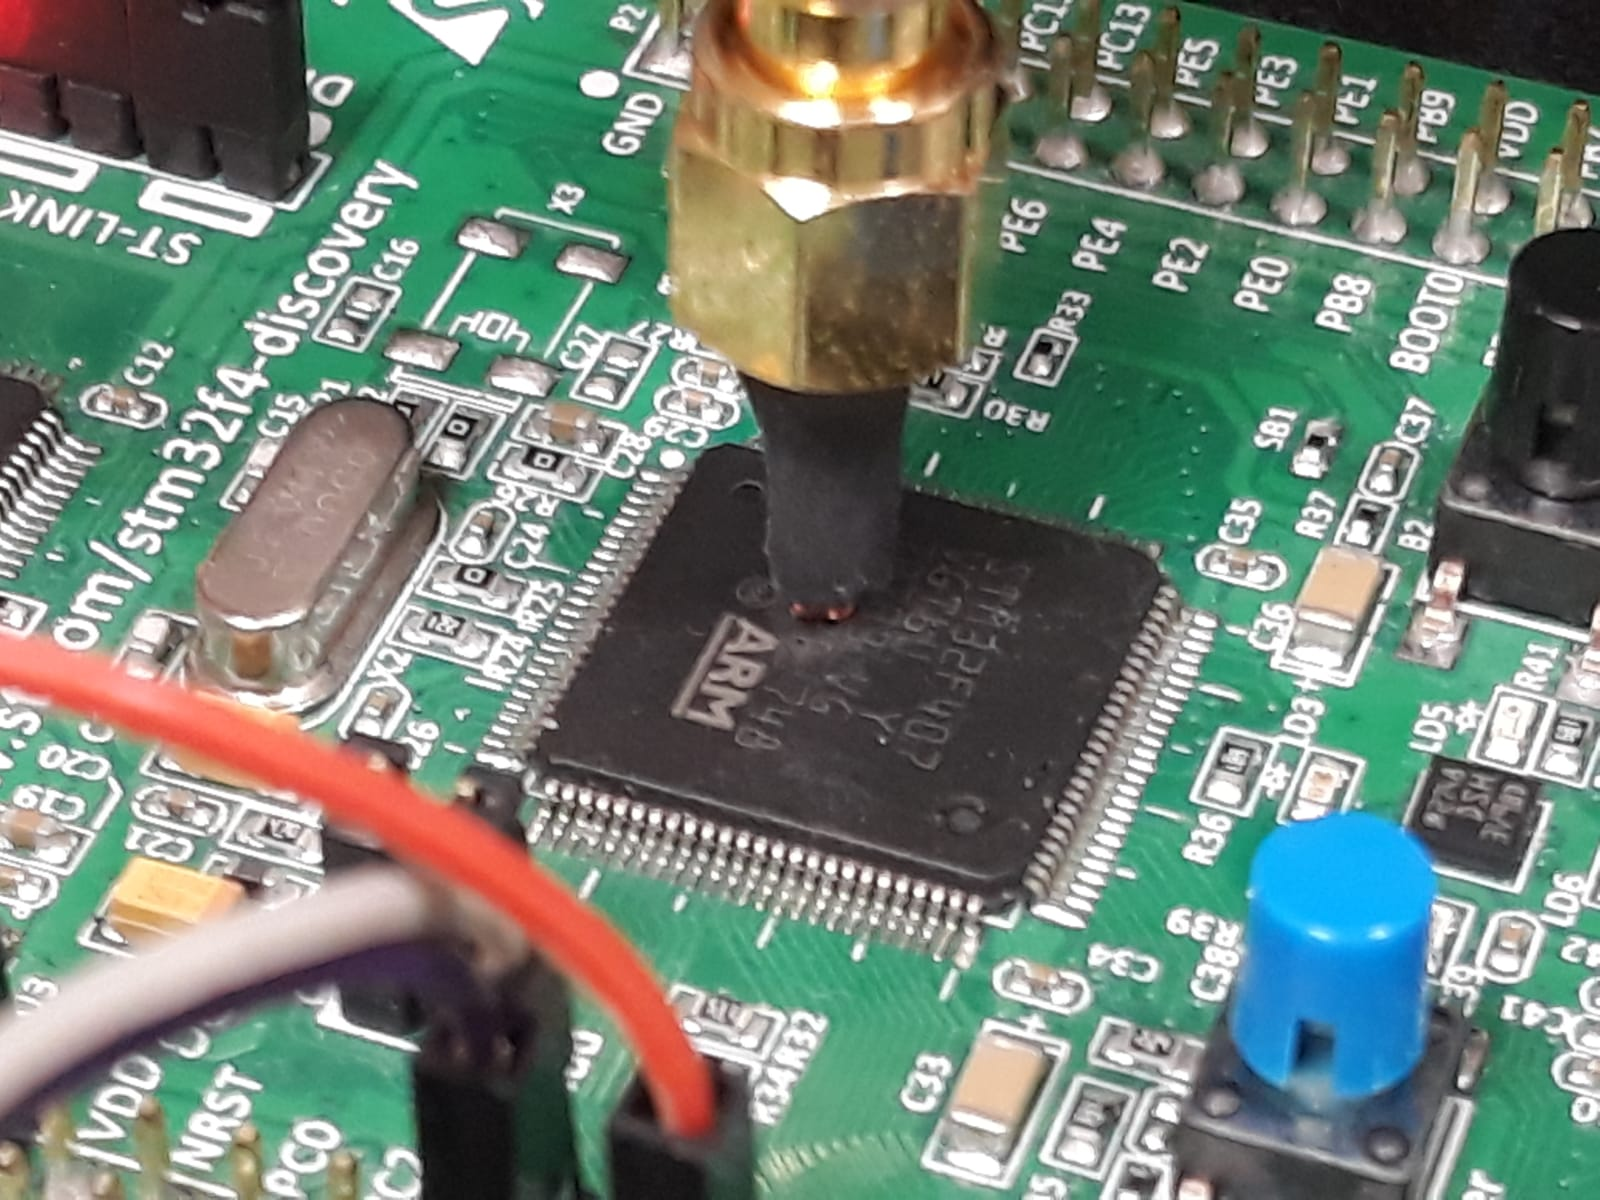
\includegraphics[width=0.5\linewidth]{./figures/fault_probe_on_chip.jpeg}
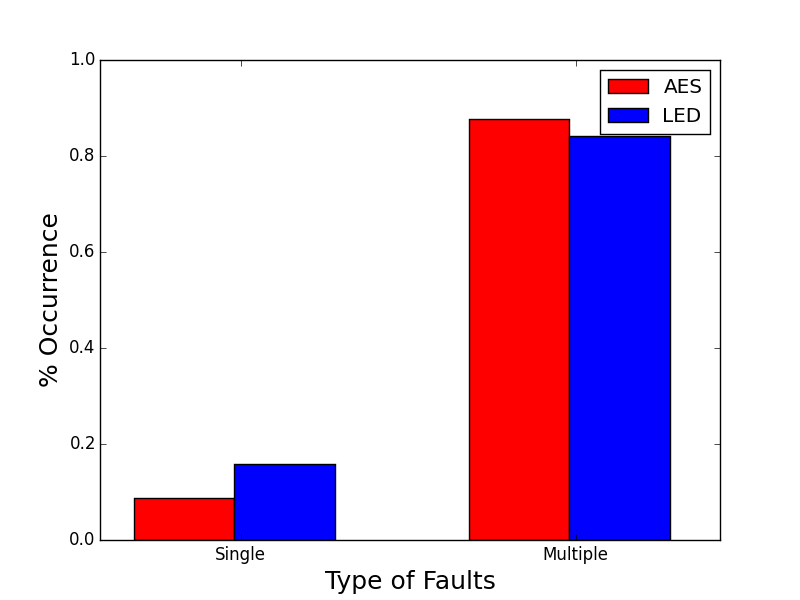
\includegraphics[width=0.65\linewidth]{./figures/faults_multiple.png}
\end{center}
\column[c]{0.5\textwidth}
\begin{center}
\visible<2>{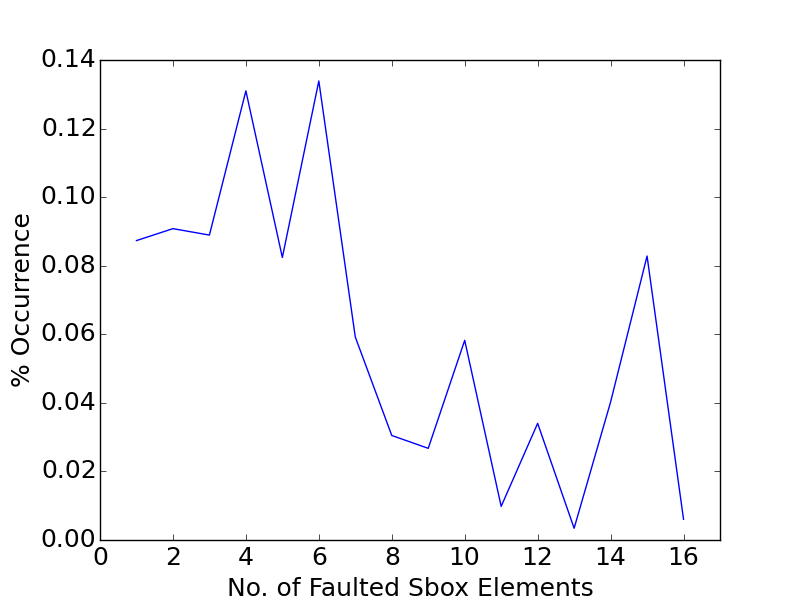
\includegraphics[width=0.65\linewidth]{./figures/faults_aes.png}}
\visible<2>{
  {\footnotesize
  \[\lambda = 6,~ N = 1526, ~|K|=256\]
  \[\text{Exp:}~\texttt{cnt}_{w} = 3197.91, ~ \texttt{cnt}_{c} = 6086.93\]
  \[\text{The:}~\texttt{cnt}_{w} = 3197.89, ~ \texttt{cnt}_{c} = 6983.73\]
  }
}
\end{center}
\end{columns}
\end{frame}

\section{Conclusion}
\sectionheader[\huge\color{tug}\faClockO]{Conclusion}

\begin{frame}{Our Main Contributions}
\begin{itemize}
\item[\faCheckCircleO] We removed the assumption of knowing the fault location in PFA
\item[\faCheckCircleO] We exploit the fault leakages in deeper rounds (until the first round)
\item[\faCheckCircleO] Our new technique decreases the number of key candidates by a factor of $\approx 2^{45}$
\item[\faCheckCircleO] Our new technique reduces the number of required ciphertexts
\end{itemize}

\begin{center}
\vspace{0.44cm}

{\large Thanks for your attention!}

\vspace{0.35cm}
\url{https://github.com/hadipourh/faultyaes}
\end{center}
\end{frame}

%%%%%%%%%%%%%%%%%%%%%%%%%%%%%%%%%%%%%%%%%%%%%%%%%%%%%%%%%%%%%%%%%%%%%%%%%%%%

\begin{frame}[allowframebreaks]{Bibliography}
  \printbibliography
\end{frame}

\begin{filecontents*}[overwrite]{\jobname.bib}

@inproceedings{eurocrypt_BonehDL97,
author    = {Dan Boneh and
				     Richard A. DeMillo and
				     Richard J. Lipton},
title     = {On the Importance of Checking Cryptographic Protocols for Faults (Extended
				Abstract)},
booktitle = {{EUROCRYPT} 1997},
series    = {Lecture Notes in Computer Science},
volume    = {1233},
pages     = {37--51},
publisher = {Springer},
year      = {1997},
doi       = {10.1007/3-540-69053-0_4}
}

@article{tches_0010L0BHDQR18,
  author    = {Fan Zhang and
               Xiaoxuan Lou and
               Xinjie Zhao and
               Shivam Bhasin and
               Wei He and
               Ruyi Ding and
               Samiya Qureshi and
               Kui Ren},
  title     = {Persistent Fault Analysis on Block Ciphers},
  journal   = {{IACR} Trans. Cryptogr. Hardw. Embed. Syst.},
  volume    = {2018},
  number    = {3},
  pages     = {150--172},
  year      = {2018},
  doi       = {10.13154/tches.v2018.i3.150-172}
}

@article{tcad_XuZYZHR21,
  author    = {Guorui Xu and
               Fan Zhang and
               Bolin Yang and
               Xinjie Zhao and
               Wei He and
               Kui Ren},
  title     = {Pushing the Limit of {PFA:} Enhanced Persistent Fault Analysis on
               Block Ciphers},
  journal   = {{IEEE} Trans. Comput. Aided Des. Integr. Circuits Syst.},
  volume    = {40},
  number    = {6},
  pages     = {1102--1116},
  year      = {2021},
  doi       = {10.1109/TCAD.2020.3048280}
}

@article{tches_ZhangZJZBZLGR20,
  author    = {Fan Zhang and
               Yiran Zhang and
               Huilong Jiang and
               Xiang Zhu and
               Shivam Bhasin and
               Xinjie Zhao and
               Zhe Liu and
               Dawu Gu and
               Kui Ren},
  title     = {Persistent Fault Attack in Practice},
  journal   = {{IACR} Trans. Cryptogr. Hardw. Embed. Syst.},
  volume    = {2020},
  number    = {2},
  pages     = {172--195},
  year      = {2020},
  doi       = {10.13154/tches.v2020.i2.172-195}
}

\end{filecontents*}

\end{document}
